\documentclass[ucs,9pt]{beamer}
\setbeamertemplate{navigation symbols}{}
% remove this line and the "ucs" option to the documentclass when your editor is not utf8-capable
\usepackage[utf8x]{inputenc}    % to make utf-8 input possible
\usepackage[english]{babel}     % hyphenation etc., alternatively use 'german' as parameter
%\usepackage{listings}

\include{fu-beamer-template}  % THIS is the line that includes the FU template!

\usepackage{arev,t1enc} % looks nicer than the standard sans-serif font
% if you experience problems, comment out the line above and change
% the documentclass option "9pt" to "10pt"

% image to be shown on the title page (without file extension, should be pdf or png)
\titleimage{mi-bildbalken}
\title[Para Sort] % (optional, use only with long paper titles)
{Paralleles Sortierung}

%\subtitle
%{Include Only If Paper Has a Subtitle}

\author[] % (optional, use only with lots of authors)
{Björn Rathjen \and Patrick Winterstein}
% - Give the names in the same order as the appear in the paper.

\institute[FU Berlin] % (optional, but mostly needed)
{Freie Universität Berlin}

\date[ProSem Algo]
{Proseminar Algorithmen, SS14}

%\subject{Theoretical Computer Science}
% This is only inserted into the PDF information catalog. Can be left
% out.

% you can redefine the text shown in the footline. use a combination of
% \insertshortauthor, \insertshortinstitute, \insertshorttitle, \insertshortdate, ...
\renewcommand{\footlinetext}{\insertshortinstitute, \insertshorttitle, \insertshortdate}

\AtBeginSection[]
{
	\begin{frame}<beamer>
		\tableofcontents[currentsection,hideothersubsubsections,hideothersubsections]
	\end{frame}
}

\begin{document}

%Titelblatt
%1
\begin{frame}[plain]
  \titlepage
\end{frame}
 
%Inhaltsverzeichnis
%2
\begin{frame}{Inhalt}
  \tableofcontents[hideallsubsubsections,allowframebreaks] %currentsection,hideallsubsections,hideallsubsubsections
  % You might wish to add the option [pausesections]
\end{frame}


% Motivation
%3
\section{Motivation}

%4  
\begin{frame}{Motivation : Allgemein}
    ist Basis für :
    \begin{itemize}
        \item Suche
        \item (Sortierung)
        \begin{itemize}
            \item Listen
            \item Wörterbücher
            \item ... 
        \end{itemize}
        \item Ist dies auch in Hardware möglich ?
    \end{itemize}
\end{frame}

%5
\section{Grundlage des Sortierens}
\subsection{Komparator}

%6
\begin{frame}{Aufbau}
    \begin{minipage}[c]{14.5cm}
    		\begin{minipage}[c]{5cm}
        		\begin{itemize}
            		\item 2 Eingänge
	            	\item vergleichender Baustein
    		        	\item 2 Ausgänge
        		\end{itemize}
	    \end{minipage}
%    		\hfill
		\begin{minipage}[c]{5cm}
			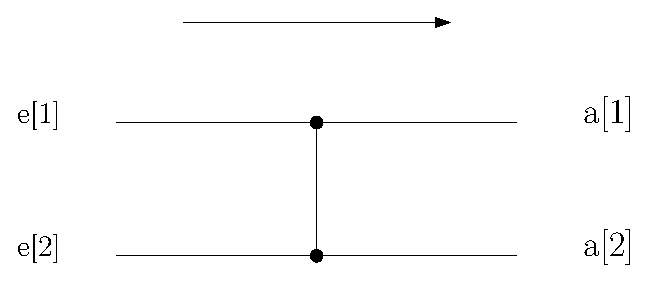
\includegraphics[scale=0.5]{Komparator1.eps}
	 	\end{minipage}
    \end{minipage}
\end{frame}

%Pseudocode
%6
\begin{frame}[fragile]{Vergleichender Baustein (ii)}
\begin{lstlisting}[laguage={inform},tabsize=4]
    void comp(chan in1, in2, out1, out2){
        a = <- in1;
        b = <- in2;
        
        if (a < b){
            out1 <- a;
            out2 <- b;
            return void;
        }
        out1 <- b;
        out2 <- a;
        return void;
    }
\end{lstlisting}
\end{frame}

%7
\section{Sortiernetzwerk}
\subsection{Aufbau}

%8
\begin{frame}{Erweiterung : Aufbau}
    \begin{itemize}
        \item mehrere Eingabeleitungen (gleiche Anzahl an Ausgabeleitungen)
        \item mehrere vergleichende Schritte
        \item Ausgabe soll sortiert sein
    \end{itemize}
\end{frame}

%9
\subsubsection*{naiver Ansatz}

%10
\begin{frame}{naiv : Aufgabe}
\uncover<1-> {Aufgabe :\\
        \begin{itemize}
            \item Resultat soll sortierte Ausgabe sein
            \end{itemize}
            }
\uncover<2-> {grundlegendes Prinzip :
        \begin{itemize}
            \item intuitiver Einsatz von Vergleichen
            \item Schrittweises sortieren
        \end{itemize}}
\end{frame}

%11
\begin{frame}{naiv : grundlegendes Prinzip}
\begin{center}
    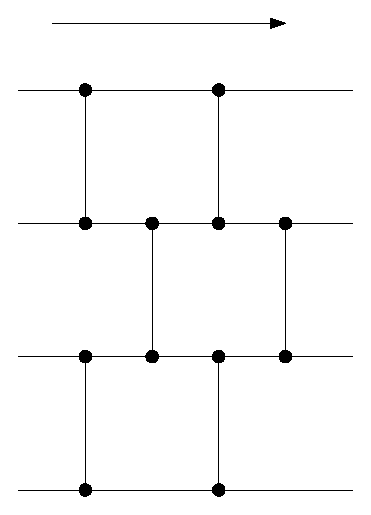
\includegraphics[scale=0.8]{bild2Komparatornetzwerk.eps}
\end{center}
\end{frame}

%12
\begin{frame}{Demonstration}
\begin{center}
   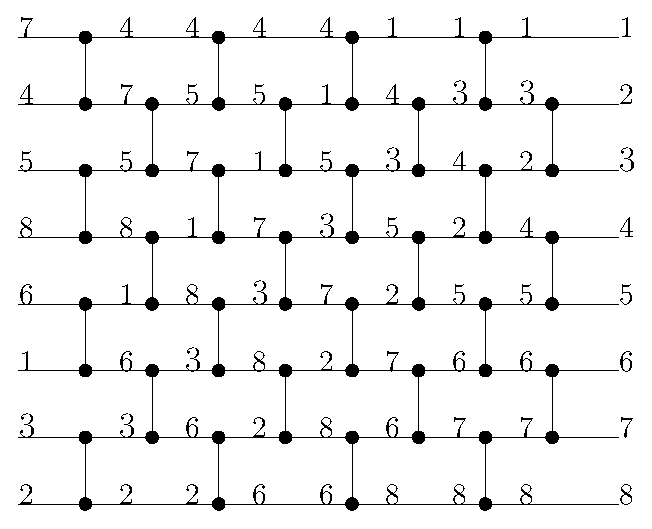
\includegraphics[scale=0.8]{bild2beispiel.eps}
  \end{center}
\end{frame}

%13
\subsection{Korrektheit}
\begin{frame}{0,1-Prinzip}
\begin{center}
Wenn es eine Folge A gibt, die ein Sortiernetzwerk nicht sortiert, so existiert auch eine 0,1-Folge, die von diesem Netzwerk nicht sortiert wird.
\end{center}
%\begin{proof}
%siehe Tafel
%\uncover<2-> Anwendung Abbildung 
%\end{proof}
\end{frame}

%14
\begin{frame}{Ansatz}
    man kann jede Zahlenfolge durch eine 0,1 Folge repräsentieren\\
    Konstante k und Zahlenfolge A mit den Elementen $a_i$\\
    $$
    f(a_i) = \begin{cases} 0 , & if \;\;a_i < k \\
    1 , & if \;\;a_i \geq k
    \end{cases}$$
\end{frame}

%15
\begin{frame}{0,1- Beispiel}
\uncover<1-> {
\begin{center}
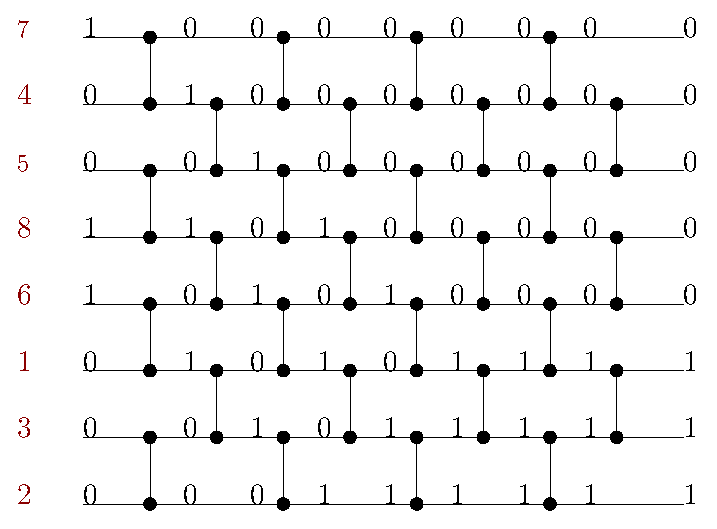
\includegraphics[scale=0.8]{01beispiel.eps}
\end{center}
}
%Bild letzte Komparatorebene weglassen
\uncover<2-> {\begin{center} {\color{green}Beispiel an der Tafel ?}\end{center} }
\end{frame}

%16
\subsection*{Aufbau eines effektieveren Netzwerks}
%Einsatzorte
\begin{frame}{effektiveres Netzwerk}
\uncover<2-> {Aufgabe :
            \begin{itemize}
                \item Resultat soll sortierte Ausgabe sein
                \item \alert{soll effizient sein}
            \end{itemize}}
\uncover<3-> {grundlegendes Prinzip :
            \begin{itemize}
                \item intuitiver Einsatz von Vergleichen
                \item[]\alert{+ Einbezug von Teile und Herrscher}
                % mh sehr leere Folien
            \end{itemize}}
\end{frame}

%17
\begin{frame}{Aufteilung}
\begin{center}
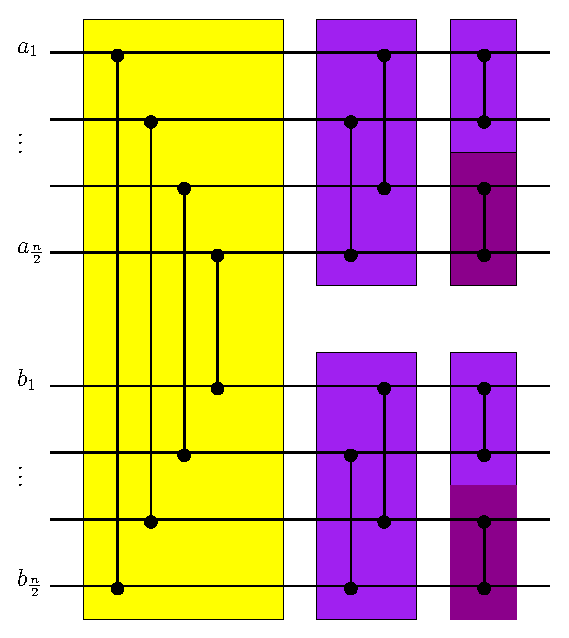
\includegraphics[scale=0.6]{bitonmischer.eps}
\end{center}
\end{frame}

%18
\begin{frame}{Bitonmischer}
Ablauf :
\begin{itemize}
\item sortierte Eingabelisten gemischt
	\begin{itemize}
	\item untere Hälfte alle größer als in oberer
	\end{itemize}
\item rekursiv die kleineren listen 
\item Resultat eine Sortierte Liste
\end{itemize}
\end{frame}

%19
\begin{frame}{odd even sort}
Ablauf :
\begin{itemize}
\item bekommen zwei sortierte Listen
\item trennen in geraden und ungeraden Index
\item fassen a(even) b(odd) = c und a(odd) b(even) = d zusammen (Resultat muss sortiert sein)
\item c und d werden indexweise verschachtelt
\item aufeinander folgende paare werden verglichen und in richtige Reihenfolge gebracht
\end{itemize}
\end{frame}

%20
\begin{frame}{Biton -Sortierer : Aufbau}
    \begin{center}
    		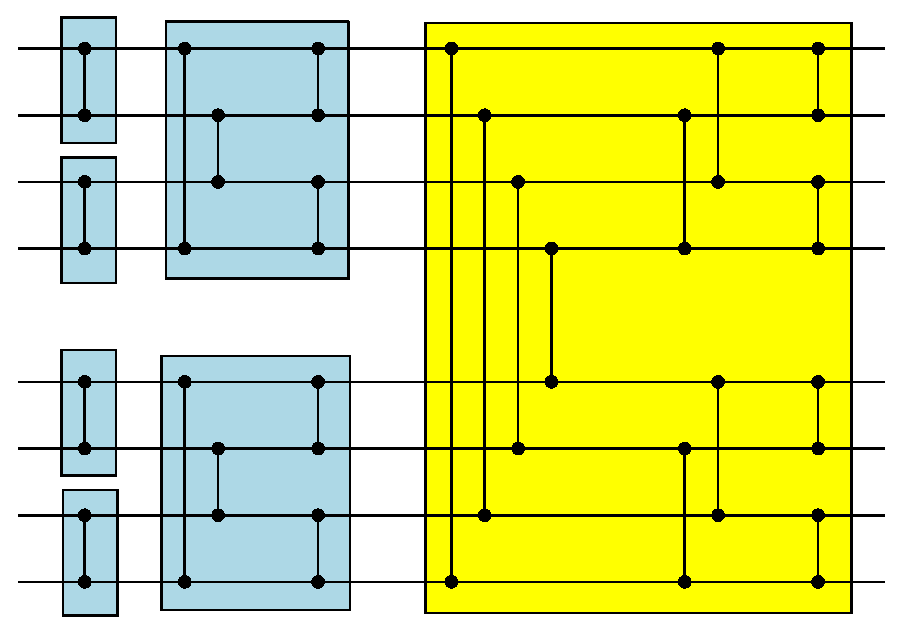
\includegraphics[scale=0.6]{biton2.eps}
    \end{center}
\end{frame}

\begin{frame}{Demonstration}
    Bild kleiner Zahlenfolge 4-8-16\\
    Beispiel
\end{frame}

%21
\section{Laufzeit}
\subsection{Herleitung}

%22
\begin{frame}{Herleitung der Laufzeit}
\begin{center}
\begin{tabular}{c|c}
%eventuell noch 2^0
N & Anzahl der Schritte \\
\hline \\
\uncover<1-> {$2^1$} & \uncover<2-> { $1$}\\
\uncover<3-> {$2^2$} & \uncover<4-> { $1 + 2$}\\
\uncover<5-> {$2^k$}& \uncover<6-> { $1 + 2 + 3 + … + k-1 + k  = \sum_{i=1}^k i$}\\
\uncover<7-> {{\color{gray}(kleiner Gauss)}} & \uncover<8-> {$ =\frac{k \cdot (k+1)}{2} $} \\
\uncover<9-> {{\color{gray}$(k = log_2 n)$}} &\uncover<10-> {$\Rightarrow \frac{1}{2}\; \cdot\;\log_2 n \;\; (\log_2 n\;+\;1)$} \\
\end{tabular}
\end{center}
\end{frame}

%23
\subsection{Vergleich mit Software sortieren}
\begin{frame}{Vergleich zu Softwareansätzen}
	\begin{itemize}
		\item Schritte gegen Vergleiche
	 	\item Abhängigkeit von der Eingabe
	 	\item Bezug zum vorherigen Vergleich
	\end{itemize}
\end{frame}

%24
\begin{frame}{Bubblesort im Hardwarenetz}
	\begin{center}
	    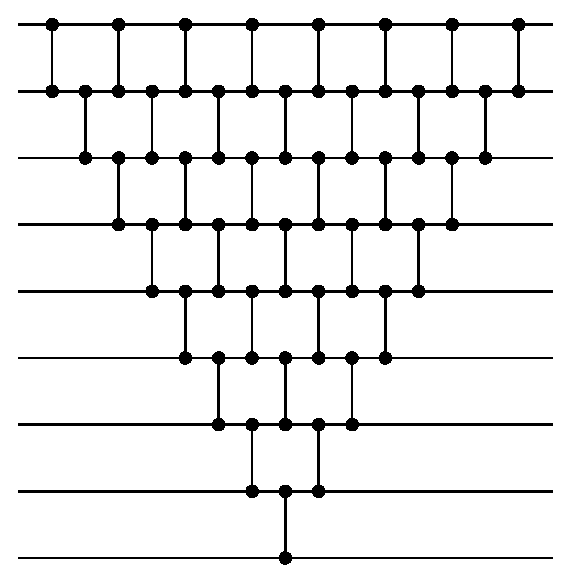
\includegraphics[scale=0.65]{bubblesort.eps}
	\end{center}
\end{frame}

%25
\begin{frame}{Softwaresortieren im Hardwarenetz}
Mergesort Quicksort
    \begin{center}
    		\includegraphics[scale=0.65]{mergesort.eps}
    		%Zeichnung 1 Pivot ist nicht auffindbar
    		%Zeichnung 2 wo war das größere Element vorher 
    		%			welcher Vergleich muss nun gemacht werden
\end{center}     
\uncover<2-> {Quichsort : wo ist das Pivot Element ?\\ Mit welchem Element müssen wir nun vergleichen?}\\
\uncover<3-> {Mergesort : Wo ist nun das größte Element ? \\welcher Vergleich kommt nun?)}
\end{frame}

%26
\section{Gegenüberstellung}
\begin{frame}
    \begin{itemize}
        \item Geschwindigkeit vs Variabilität
        \begin{itemize}
            \item hohe Geschwindigkeit durch direkte Hardware Implementriegung
            \item starre Struktur , bildet Rahmen der Möglichkeiten
            \item stark typisierte Eingabe
        \end{itemize}
    \item Hardwareaufwand vs Softwareaufwand
        \begin{itemize}
            \item Software zur Auswertung keine zum sortieren
            \item geringe Skalierbarkeit
            \item hoher Aufwand wenn Eingabelimit überschritten wird
            \item nur lokal
            \item Hardware Konzeption eventuell aufwendiger
        \end{itemize}
    \end{itemize}
\end{frame}

%27
\section{Zusammenfassung}
\begin{frame}{Zusammenfassung}
\begin{itemize}
  \item paralleles sortieren ist schnell und effizient 
  \item problemabhängige Lösung
  \item starr, nicht universell
\end{itemize}
\end{frame}

%28
\section{Ausblick}
\begin{frame}{Ausblick}
\begin{itemize}
\item andere Arten von Netzwerken
\item Hypercubes
\item Simulation von Maschinenmodellen
\item …
\end{itemize}
\end{frame}


<<<<<<< HEAD
%29
=======
\begin{frame}{Aufbau}
structure
\end{frame}

\begin{frame}{Funktion}

\end{frame}

%Ende
\begin{frame}{Ende}
    Fragen, Anregungen?\\
    (keine Liederwünsche)
\end{frame}

>>>>>>> branch 'master' of https://github.com/gravion/CoursesSS14
\subsection{Anhang}
\appendix
\section<presentation>*{\appendixname}
\subsection<presentation>*{For Further Reading}

\begin{frame}[allowframebreaks]
  \frametitle<presentation>{For Further Reading}
    
  \begin{thebibliography}{10}
    
  \beamertemplatebookbibitems
  % Start with overview books.

  \bibitem{}
    A.~Author.
    \newblock {\em Taschenbuch der Algorithmen}.
    \newblock Springer Verlag , 2008.
    
  \bibitem{Author1990}
    Tom Leighton.
    \newblock {\em Einführung in Parallele Algorithmen und Architekturen}{\\Gitter, Bäume und Hypercubes}.
    \newblock Thomsom Publisching , 1997.
 
    
  \beamertemplatearticlebibitems
  % Followed by interesting articles. Keep the list short. 

  \bibitem{0,1-Prinzip}
    S.~Someone.
   % \href{http://www.iti.fh-flensburg.de/lang/algorithmen/sortieren/networks/nulleins.htm}
    \newblock 
    \newblock {http://www.iti.fh-flensburg.de/lang/algorithmen/sortieren/networks/nulleins.htm}
    
  \end{thebibliography}
\end{frame}


%%%%%%%%%%%%%%%%%%%%%%%%%%%%%%%%%%%%%%%%%%%%%%%%%%%%%%%%%%%%%%%%%%%%%%%%%%%%%%%%%%%%%%%%%%%%

\end{document}


\subsection{Hybercube}
\begin{frame}{Hyprecube}
?¿
\end{frame}

\begin{frame}{Aufbau}
structur
\end{frame}

\begin{frame}{Funktion}

\end{frame}

%Ende
\begin{frame}{Ende}
    Fragen, Anregungen?\\
    (keine Liederwünsche)
\end{frame}

\begin{frame}{Make Titles Informative. Use Uppercase Letters. Long Titles are Split Automatically.}{Subtitles are optional.}
  % - A title should summarize the slide in an understandable fashion
  %   for anyone how does not follow everything on the slide itself.
  \begin{itemize}
  \item
    Use \texttt{itemize} a lot.
  \item
   	Kurze Sätze benutzen.
  \end{itemize}
\end{frame}

\begin{frame}{Make Titles Informative.}

  You can create overlays\dots
  \begin{itemize}
  \item using the \texttt{pause} command:
    \begin{itemize}
    \item
      First item.
      \pause
    \item    
      Second item.
    \end{itemize}
  \item
    using overlay specifications:
    \begin{itemize}
    \item<3->
      First item.
    \item<4->
      Second item.
    \end{itemize}
  \item
    using the general \texttt{uncover} command:
    \begin{itemize}
      \uncover<5->{\item
        First item.}
      \uncover<6->{\item
        Second item.}
    \end{itemize}
  \end{itemize}
\end{frame}

\begin{frame}[fragile]{An old algorithm}
% NB. listings is quite powerful, but not well suited to be used with beamer
%  consider using semiverbatim or the like, see below
\begin{lstlisting}[language=C]
int main (void)
{
  std::vector<bool> is_prime (100, true);
  for (int i = 2; i < 100; i++)
    if (is_prime[i])
      {
        std::cout << i << " ";
        for (int j = i; j < 100;
            is_prime [j] = false, j+=i);
      }
  return 0;
}
\end{lstlisting}
\end{frame}

\begin{frame}[fragile]
  \frametitle{An Algorithm For Finding Primes Numbers.}
\begin{semiverbatim}
\uncover<1->{\alert<0>{int main (void)}}
\uncover<1->{\alert<0>{\{}}
\uncover<1->{\alert<1>{ \alert<4>{std::}vector<bool> is_prime (100, true);}}
\uncover<1->{\alert<1>{ for (int i = 2; i < 100; i++)}}
\uncover<2->{\alert<2>{    if (is_prime[i])}}
\uncover<2->{\alert<0>{      \{}}
\uncover<3->{\alert<3>{        \alert<4>{std::}cout << i << " ";}}
\uncover<3->{\alert<3>{        for (int j = i; j < 100;}}
\uncover<3->{\alert<3>{             is_prime [j] = false, j+=i);}}
\uncover<2->{\alert<0>{      \}}}
\uncover<1->{\alert<0>{ return 0;}}
\uncover<1->{\alert<0>{\}}}
\end{semiverbatim}
  \visible<4->{Note the use of \alert{\texttt{std::}}.}
\end{frame}



\begin{frame}{Make Titles Informative.}
  \begin{example}
    \begin{itemize}
    \item 2 is prime (two divisors: 1 and 2).
    \item 3 is prime (two divisors: 1 and 3).
    \item 4 is not prime (\alert{three} divisors: 1, 2, and 4).
    \end{itemize}
  \end{example}
\end{frame}

\begin{frame}{Make Titles Informative.}
\begin{theorem}
 There is no largest prime number and, in addition, $$\int_\Omega \nabla u \cdot \nabla v = - \int_\Omega u \Delta v + \int_{\partial\Omega} u v n$$
 \end{theorem}
 \begin{proof}
 \begin{enumerate}
 \item<1-> Suppose $p$ were the largest prime number.
 \item<2-> Let $q$ be the product of the first $p$ numbers.
 \item<3-> Then $q + 1$ is not divisible by any of them.
 \item<1-> Thus $q + 1$ is also prime and greater than $p$.\qedhere
 \end{enumerate} 
 \end{proof}
 \uncover<4->{The proof used \textit{reductio ad absurdum}.}
\end{frame}

\begin{frame}{Make Titles Informative.}
\end{frame}



\begin{frame}{Summary}

  % Keep the summary *very short*.
  \begin{itemize}
  \item
    The \alert{first main message} of your talk in one or two lines.
  \item
    The \alert{second main message} of your talk in one or two lines.
  \item
    Perhaps a \alert{third message}, but not more than that.
  \end{itemize}
  
  % The following outlook is optional.
  \vskip0pt plus.5fill
  \begin{itemize}
  \item
    Outlook
    \begin{itemize}
    \item
      Something you haven't solved.
    \item
      Something else you haven't solved.
    \end{itemize}
  \end{itemize}
\end{frame}
